\documentclass[11pt]{article}

\usepackage[a4paper,margin=1in]{geometry}
\usepackage[T1]{fontenc}
\usepackage[utf8]{inputenc}
\usepackage{lmodern}
\usepackage{amsmath,amssymb,mathtools}
\usepackage{bm}
\usepackage{booktabs}
\usepackage{graphicx}
\usepackage{hyperref}
\usepackage{xcolor}

\hypersetup{
  colorlinks=true,
  linkcolor=blue!60!black,
  citecolor=blue!60!black,
  urlcolor=blue!60!black
}

\newcommand{\Ds}{D_s}
\newcommand{\Dsone}{D_{s1}}
\newcommand{\GeV}{\mathrm{GeV}}
\newcommand{\ii}{\mathrm{i}}
\newcommand{\ee}{\mathrm{e}}
\newcommand{\Tr}{\mathrm{Tr}}
\newcommand{\slashp}[1]{#1\!\!\!/}
\newcommand{\qbar}{\bar q}
\newcommand{\sbar}{\bar s}
\newcommand{\vev}[1]{\left\langle #1 \right\rangle}

\title{Working Notes for $\Dsone \to \Ds \gamma$ in Light-Cone QCD Sum Rules}
\author{Ds gamma project}
\date{\today}

\begin{document}
\maketitle

\begin{abstract}
These notes are a living derivation for the light-cone QCD sum-rule
calculation of $\Dsone(2460)\to\Ds\gamma$ and
$\Dsone(2536)\to\Ds\gamma$.  The purpose is pedagogical as well as practical:
each step is written so that a master's student can follow the choices,
conventions, and algebra before the final paper-level formulas are assembled.
\end{abstract}

\section{Conventions}

We use the mostly-minus metric
\begin{equation}
  g_{\mu\nu}=\mathrm{diag}(+1,-1,-1,-1),
\end{equation}
and
\begin{equation}
  \{\gamma_\mu,\gamma_\nu\}=2g_{\mu\nu},\qquad
  \sigma_{\mu\nu}=\frac{\ii}{2}[\gamma_\mu,\gamma_\nu],
  \qquad
  \gamma_5=\ii\gamma^0\gamma^1\gamma^2\gamma^3 .
\end{equation}
The Levi-Civita convention is
\begin{equation}
  \epsilon^{0123}=+1,\qquad \epsilon_{0123}=-1,
\end{equation}
so that
\begin{equation}
  \Tr[\gamma_5\gamma_\mu\gamma_\nu\gamma_\alpha\gamma_\beta]
  =-4\ii\,\epsilon_{\mu\nu\alpha\beta}.
\end{equation}
Our Fourier convention for a propagator is
\begin{equation}
  S(x)=\int\frac{d^4 k}{(2\pi)^4}\,\ee^{-\ii k\cdot x}\,\widetilde S(k).
\end{equation}

\section{Currents and Momentum Assignment}

The external momenta are
\begin{equation}
  P=p+q,
\end{equation}
where $P$ is the initial axial-meson momentum, $p$ is the final pseudoscalar
$\Ds$ momentum, and $q$ is the real-photon momentum.

The pseudoscalar interpolating current is
\begin{equation}
  J_{\Ds}(x)=\sbar(x)\,\ii\gamma_5\,Q(x).
\end{equation}
For the axial channel we use two independent currents,
\begin{align}
  J^{(0)}_{A\mu}(x)
  &= \sbar(x)\gamma_\mu\gamma_5 Q(x),\\
  J^{(0)}_{B\mu}(x)
  &= \frac{\ii}{m_Q+m_s}\,
     \sbar(x)\sigma_{\mu\alpha}P^\alpha\gamma_5 Q(x).
\end{align}
The tensor current contracts with $P^\alpha$, not $p^\alpha$, because it
interpolates the initial axial state.  The factor $1/(m_Q+m_s)$ restores the
same mass dimension as the axial-vector current.

\section{Correlation Function}

For a generic axial current $\Gamma_\mu\in\{\gamma_\mu\gamma_5,\,
\ii\sigma_{\mu\alpha}P^\alpha\gamma_5/(m_Q+m_s)\}$ we study
\begin{equation}
  \Pi_\mu(p,q)
  =
  \ii\int d^4x\,\ee^{\ii p\cdot x}
  \langle \gamma(q,\varepsilon)|
  T\{ \sbar(x)\Gamma_\mu Q(x)\,
       \bar Q(0)\ii\gamma_5 s(0)\}
  |0\rangle .
  \label{eq:correlator}
\end{equation}
The target Lorentz structure for the $1^+\to0^-\gamma$ transition is
\begin{equation}
  (\eta\cdot\varepsilon^*)(p\cdot q)
  -(\eta\cdot q)(p\cdot\varepsilon^*).
\end{equation}
On the correlator side we therefore project onto an equivalent transverse
structure built from the open axial index and the photon polarization.
With open indices this structure is represented by
\begin{equation}
  T_{\mu\nu}=(p\cdot q)g_{\mu\nu}-q_\mu p_\nu,
  \qquad
  S_{\mu\nu}\equiv -T_{\mu\nu}=p_\nu q_\mu-(p\cdot q)g_{\mu\nu}.
\end{equation}
For a real photon, $q^2=0$, it obeys
\begin{equation}
  q^\nu S_{\mu\nu}=0,
\end{equation}
so the projected invariant amplitude is gauge invariant under
$\varepsilon_\nu\to\varepsilon_\nu+\lambda q_\nu$.  In scalar form the same
statement is
\begin{equation}
  (\eta\cdot q)(p\cdot q)-(\eta\cdot q)(p\cdot q)=0
\end{equation}
after replacing $\varepsilon\to q$.

\section{Wick Contraction and OPE Bookkeeping}

The OPE is separated into a hard-photon sector and a soft-photon sector:
\begin{equation}
  \Pi_\mu^{\mathrm{OPE}}
  =
  \Pi_\mu^{\mathrm{hard}}
  +
  \Pi_\mu^{\mathrm{soft}}.
\end{equation}
This split is important because the two terms describe different physics and
must not be double counted.

\subsection{Hard photon emission}

In the hard sector the photon is emitted perturbatively from either the heavy
quark or the strange quark.  After Wick contraction one obtains
\begin{equation}
  \Pi_\mu^{\mathrm{hard}}
  =
  \ii N_c\int d^4x\,\ee^{\ii p\cdot x}
  \Tr_D\!\left[
    \Gamma_\mu S_Q^\gamma(x)\,\ii\gamma_5\,S_s^0(-x)
    +
    \Gamma_\mu S_Q^0(x)\,\ii\gamma_5\,S_s^\gamma(-x)
  \right],
  \label{eq:hard-wick}
\end{equation}
where $N_c=3$ and $\Tr_D$ denotes the Dirac trace.  The free massive propagator is
\begin{equation}
  S_q^0(x)
  =
  \int\frac{d^4k}{(2\pi)^4}\,\ee^{-\ii k\cdot x}
  \frac{\ii(\slashp{k}+m_q)}{k^2-m_q^2}.
\end{equation}
We keep explicit powers of $m_s$, including possible $m_s^2$ terms.

The first-order electromagnetic background-field correction for a generic quark
flavor $q$ is
\begin{align}
  S_q^\gamma(x)
  &=
  -\ii e_q
  \int\frac{d^4k}{(2\pi)^4}\,\ee^{-\ii k\cdot x}
  \int_0^1du
  \Bigg[
    \frac{\slashp{k}+m_q}{2(m_q^2-k^2)^2}
    F^{\alpha\beta}(ux)\sigma_{\alpha\beta}
    +
    \frac{u x_\alpha}{m_q^2-k^2}
    F^{\alpha\beta}(ux)\gamma_\beta
  \Bigg].
  \label{eq:em-propagator}
\end{align}
In Eq.~\eqref{eq:hard-wick} this generic formula is used twice:
\begin{align}
  S_Q^\gamma(x)
  &= S_q^\gamma(x)\big|_{q\to Q,\;m_q\to m_Q,\;e_q\to e_Q},\\
  S_s^\gamma(x)
  &= S_q^\gamma(x)\big|_{q\to s,\;m_q\to m_s,\;e_q\to e_s}.
\end{align}
Thus the hard sector contains both heavy-line and strange-line electromagnetic
background-field insertions.
For a real photon we write
\begin{equation}
  F^{\alpha\beta}(ux)
  =
  \ii(\varepsilon^\alpha q^\beta-\varepsilon^\beta q^\alpha)
  \ee^{\ii u q\cdot x},
\end{equation}
with the overall phase kept consistent with the Fourier convention.

Equation~\eqref{eq:em-propagator} is not a vacuum-condensate correction.  It is
the quark propagator in an external electromagnetic field and is included in
the base analysis.  What we do not include in the base hard sector are the
ordinary SVZ-style condensate-expanded propagator terms such as
$\langle\bar s s\rangle$, $\langle\bar s g_s\sigma Gs\rangle$, or
$\langle G^2\rangle$ propagator corrections.

\subsection{Equivalent momentum-space vertex form}

For FeynCalc trace checks it is often simpler to use the equivalent explicit
photon-vertex representation.  With photon index $\nu$,
\begin{align}
  N_{Q,\mu\nu}
  &=
  \Tr_D\!\left[
    \Gamma_\mu
    (\slashp{k}+\slashp{q}+m_Q)
    \gamma_\nu
    (\slashp{k}+m_Q)
    \ii\gamma_5
    (\slashp{k}-\slashp{p}+m_s)
  \right],
  \\
  N_{s,\mu\nu}
  &=
  \Tr_D\!\left[
    \Gamma_\mu
    (\slashp{k}+m_Q)
    \ii\gamma_5
    (\slashp{k}-\slashp{p}+m_s)
    \gamma_\nu
    (\slashp{k}-\slashp{p}+\slashp{q}+m_s)
  \right].
\end{align}
These numerators are accompanied by the denominators
\begin{align}
  D_Q &=
  [(k+q)^2-m_Q^2][k^2-m_Q^2][(k-p)^2-m_s^2],\\
  D_s &=
  [k^2-m_Q^2][(k-p)^2-m_s^2][(k-p+q)^2-m_s^2].
\end{align}
The explicit-vertex form and the background-field form represent the same hard
emission physics.  We must not add both as independent contributions.

\subsection{Soft photon emission: two-particle photon DAs}

In the soft sector the photon is represented by its light-cone distribution
amplitudes.  Contracting only the heavy quark gives
\begin{equation}
  \Pi_\mu^{\mathrm{soft},2p}
  =
  \ii\int d^4x\,\ee^{\ii p\cdot x}
  [\Gamma_\mu S_Q^0(x)\ii\gamma_5]_{\alpha\beta}
  \langle\gamma(q,\varepsilon)|
  \sbar_\alpha(x)s_\beta(0)
  |0\rangle .
\end{equation}
Fierz rearrangement converts the open spinor indices to a basis of Dirac
bilinears,
\begin{equation}
  \sbar_\alpha(x)s_\beta(0)
  =
  -\frac14\sum_i(\Gamma_i)_{\beta\alpha}
  \sbar(x)\Gamma_i s(0),
\end{equation}
so that
\begin{equation}
  \Pi_\mu^{\mathrm{soft},2p}
  =
  -\frac{\ii}{4}
  \int d^4x\,\ee^{\ii p\cdot x}
  \sum_i
  \Tr_D[\Gamma_\mu S_Q^0(x)\ii\gamma_5\Gamma_i]\,
  \langle\gamma(q,\varepsilon)|
  \sbar(x)\Gamma_i s(0)
  |0\rangle .
\end{equation}
The photon matrix elements are then expressed in terms of two-particle photon
DAs.  Parameters such as $\chi\langle\bar s s\rangle$ enter here as part of the
photon wavefunction normalization; they are not condensate corrections to the
hard propagator.

\subsection{Soft photon emission: three-particle photon DAs}

To include three-particle photon DAs we must also allow one background gluon to
come from the heavy-quark propagator,
\begin{align}
  S_Q^G(x)
  &=
  -\ii g_s
  \int\frac{d^4k}{(2\pi)^4}\,\ee^{-\ii k\cdot x}
  \int_0^1du
  \Bigg[
    \frac{\slashp{k}+m_Q}{2(m_Q^2-k^2)^2}
    G^{\alpha\beta}(ux)\sigma_{\alpha\beta}
    +
    \frac{u x_\alpha}{m_Q^2-k^2}
    G^{\alpha\beta}(ux)\gamma_\beta
  \Bigg].
  \label{eq:gluon-propagator}
\end{align}
This term is not a gluon-condensate correction.  It is an operator insertion
that combines with photon matrix elements of the form
\begin{equation}
  \langle\gamma(q,\varepsilon)|
  \sbar(x)\Gamma_i g_sG_{\alpha\beta}(ux)s(0)
  |0\rangle ,
\end{equation}
which define the three-particle photon DAs.

\section{Staged Calculation Plan}

We proceed in two stages.

\paragraph{Stage 1.}
Include the hard photon emission terms and the two-particle photon DAs:
\begin{equation}
  \Pi_\mu^{\mathrm{Stage\ 1}}
  =
  \Pi_\mu^{\mathrm{hard}}
  +
  \Pi_\mu^{\mathrm{soft},2p}.
\end{equation}
This stage keeps all explicit $m_s$ terms and omits ordinary
condensate-expanded propagators.

\paragraph{Stage 2.}
Add the three-particle photon DA contributions generated by
$S_Q^G$ and the corresponding light-cone matrix elements:
\begin{equation}
  \Pi_\mu^{\mathrm{Stage\ 2}}
  =
  \Pi_\mu^{\mathrm{Stage\ 1}}
  +
  \Pi_\mu^{\mathrm{soft},3p}.
\end{equation}
This staging keeps the derivation auditable: first we verify the core hard and
two-particle DA structures, then we add the more involved background-gluon
terms.

\section{Current FeynCalc Artifacts}

The script \texttt{scripts/step2\_current\_building\_blocks.wl} checks the
basic Dirac conventions and defines the current vertices.  The script
\texttt{scripts/step2\_hard\_photon\_numerators.wl} computes numerator-level
hard-photon traces in the explicit photon-vertex representation.  These traces
are stored in \texttt{outputs/step2\_hard\_photon\_numerators.txt}.

The script \texttt{scripts/step2\_e1\_project\_hard\_numerators.wl} applies the
E1 projector
\begin{equation}
  {\cal P}^{\mu\nu}_{E1}
  =
  \frac{p^\nu q^\mu-(p\cdot q)g^{\mu\nu}}{2(p\cdot q)^2},
\end{equation}
which satisfies ${\cal P}_{E1}^{\mu\nu}
[p_\nu q_\mu-(p\cdot q)g_{\mu\nu}]=1$ for $q^2=0$.  The projected hard
numerators are stored in
\texttt{outputs/step2\_e1\_projected\_hard\_numerators.txt}.

The companion script \texttt{scripts/ward\_transversality\_check.wl} verifies
the Ward/transversality properties of the same E1 tensor with FeynCalc.  Its
output is stored in
\texttt{outputs/ward\_transversality\_check.txt}.

The script \texttt{scripts/step2\_soft\_2p\_fierz\_traces.wl} computes the
trace factors multiplying the two-particle photon DA matrix elements after the
Fierz rearrangement.  The output
\texttt{outputs/step2\_soft\_2p\_fierz\_traces.txt} shows which bilinears feed
the axial current and which feed the tensor current.

\section{Stage 1 Axial-Current Numerical Baseline}

Before deriving the tensor-current sum rule, we implemented the known
single-axial-current result for
$D_{s1}(2460)\to D_s\gamma$ as a benchmark.  This is the coupling called
$g_1$ by Colangelo, De Fazio, and Ozpineci.  In our notation this is the
axial-current form factor $G_A$.

The Stage 1 version contains
\begin{equation}
  G_A^{\mathrm{Stage\ 1}}
  =
  G_A^{\mathrm{pert}}
  +
  G_A^{\chi\phi_\gamma}
  +
  G_A^{\mathbb A,\bar H_\gamma}
  +
  G_A^{f_{3\gamma}\Psi^v},
\end{equation}
where the three-particle DA integral usually denoted by ${\cal F}_1$ is omitted
until Stage 2.

The numerical script is
\begin{center}
  \texttt{scripts/stage1\_axial\_g1\_baseline.py}.
\end{center}
It writes the full Borel/threshold grid to
\begin{center}
  \texttt{outputs/stage1\_axial\_g1\_baseline.csv}.
\end{center}

\subsection{Magnetic-susceptibility sign convention}

The Colangelo paper prints $\chi=-(3.15\pm0.30)\,\mathrm{GeV}^{-2}$ in its
matrix-element convention.  In this project we store the BBK magnitude as
\begin{equation}
  \chi(1\,\mathrm{GeV})=+3.15\pm0.30\,\mathrm{GeV}^{-2}.
\end{equation}
Therefore the sign of the $\chi\phi_\gamma$ term in the implemented sum rule is
flipped relative to the literal printed formula.  This is a convention
translation, not a physical change.  A diagnostic run that inserts positive
$\chi$ into the printed negative-$\chi$ formula gives a much larger width and is
kept only as a warning check.

\subsection{Preliminary Stage 1 result}

Using the project inputs, $u_0=1/2$, $3\le M^2\le6\,\mathrm{GeV}^2$, and
$s_0=(2.50,2.55,2.60)^2\,\mathrm{GeV}^2$, the axial-current Stage 1 grid gives
\begin{equation}
  -0.399 \le G_A^{\mathrm{Stage\ 1}} \le -0.314\quad \mathrm{GeV}^{-1}.
\end{equation}
With
\begin{equation}
  \Gamma=\frac{\alpha_{\rm em}}{3}G^2|\vec q_\gamma|^3,
\end{equation}
this corresponds to
\begin{equation}
  20.8\,\mathrm{keV}
  \le
  \Gamma_A^{\mathrm{Stage\ 1}}[D_{s1}(2460)\to D_s\gamma]
  \le
  33.5\,\mathrm{keV}.
\end{equation}
This is not yet the physical mixed-state result.  It is the axial-current
baseline that will be combined with the tensor-current form factor after the
$J_B$ sum rule is derived.

\section{First Tensor-Current Step: Leading-Twist Soft Contribution}

The tensor-current calculation starts from the trace-level identity produced by
\texttt{scripts/step3\_soft\_2p\_e1\_projection.wl}.  For the two-particle
tensor photon DA matrix element, the E1 projections are
\begin{align}
  {\cal P}_{E1}\!\left[
    \Tr(J_A\,S_Q\,i\gamma_5\,\sigma_{\rho\lambda})
    (\varepsilon^\rho q^\lambda-\varepsilon^\lambda q^\rho)
  \right]
  &=
  8\,\frac{k\cdot q}{p\cdot q},\\
  {\cal P}_{E1}\!\left[
    \Tr(J_B\,S_Q\,i\gamma_5\,\sigma_{\rho\lambda})
    (\varepsilon^\rho q^\lambda-\varepsilon^\lambda q^\rho)
  \right]
  &=
  8\,\frac{m_Q}{m_Q+m_s}.
\end{align}
After the two-particle DA Fourier integral and double Borel transform,
$k=p+\bar u q$, hence $k\cdot q=p\cdot q$ for $q^2=0$.  Therefore, before the
hadronic decay-constant normalization, the leading-twist tensor-current OPE
piece is
\begin{equation}
  \Pi_{B}^{\chi\phi_\gamma}
  =
  \frac{m_Q}{m_Q+m_s}\,
  \Pi_{A}^{\chi\phi_\gamma}.
\end{equation}

The exploratory script
\texttt{scripts/stage1\_tensor\_gb\_leading\_twist.py} uses this relation to
estimate only the $\chi\phi_\gamma$ part of $G_B$.  This is not the final
tensor-current sum rule.  It omits the tensor-current hard contribution, the
vector DA contribution, and the Stage 2 three-particle DA terms.

Using the project inputs, the partial leading-twist estimate gives
\begin{align}
  G_B^{\chi\phi_\gamma}
  &\simeq +0.205\text{ to }+0.273\ \mathrm{GeV}^{-1},
  &&\text{if } f_B=f_T,\\
  G_B^{\chi\phi_\gamma}
  &\simeq +0.114\text{ to }+0.151\ \mathrm{GeV}^{-1},
  &&\text{if } f_B=f_T\,\frac{m_{D_{s1}}}{m_c+m_s}.
\end{align}
The sizeable sign difference relative to $G_A$ means that the physical mixed
amplitudes can be sensitive to the tensor-current normalization.  This is why
the next step is to finish the full $G_B$ sum rule before quoting final mixed
widths.

\section{Decay-Constant Normalization Before Mixing}

The labels $f_A$, $f_B$, and $f_T$ must not be mixed casually.  The axial
current couples to the axial basis state through
\begin{equation}
  \langle 0|J_A^\mu|D_{s1}^{A}(P,\eta)\rangle
  =
  f_A m_A \eta^\mu ,
\end{equation}
whereas our tensor-derived current is
\begin{equation}
  J_B^\mu
  =
  \frac{\ii}{m_c+m_s}\,
  \bar s\sigma^{\mu\alpha}P_\alpha\gamma_5 c .
\end{equation}
The corresponding decay constant is defined by
\begin{equation}
  \langle 0|J_B^\mu|D_{s1}^{B}(P,\eta)\rangle
  =
  f_B m_B \eta^\mu .
\end{equation}
Therefore $f_B=f_T$ is not a physical statement by itself.  It is only true if
the tabulated $f_T$ is already defined for the same current $J_B^\mu$ and with
the same mass normalization.  If instead the input table gives the more common
tensor-current matrix element
\begin{equation}
  \langle 0|\bar s\sigma_{\mu\nu}\gamma_5 c|D_{s1}^{B}(P,\eta)\rangle
  =
  f_T(\eta_\mu P_\nu-\eta_\nu P_\mu),
\end{equation}
then contraction with $P^\nu/(m_c+m_s)$ gives the effective normalization
\begin{equation}
  f_B^{\rm eff}
  \simeq
  f_T\,\frac{m_{D_{s1}}}{m_c+m_s},
\end{equation}
up to the sign fixed by the precise convention for
$\sigma_{\mu\nu}\gamma_5$ and by the transverse condition $\eta\cdot P=0$.

Only after $G_A$ and $G_B$ have been computed with their own basis-current
decay constants do we form the physical amplitudes:
\begin{align}
  G_{2460}
  &=
  \sin\theta\,G_A+\cos\theta\,G_B,\\
  G_{2536}
  &=
  \cos\theta\,G_A-\sin\theta\,G_B.
\end{align}
Thus the sine--cosine factors belong to the physical-state mixing of amplitudes,
not to an arbitrary identification $f_B=f_T$.  In the numerical scripts,
$f_B=f_T$ is kept only as a diagnostic.  The converted
$f_B=f_T m_{D_{s1}}/(m_c+m_s)$ option is the safer central normalization unless
the input-table definition of $f_T$ is changed.

\section{Tensor-Current Hard Term: Triangle Reduction}

The hard tensor-current numerator is more complicated than the axial one because
the $J_B$ current introduces an extra factor of $P^\alpha$ and therefore higher
powers of the loop momentum after E1 projection.  The script
\texttt{scripts/step3\_tensor\_hard\_triangle\_reduction.wl} rewrites scalar
products such as $k^2$, $k\cdot p$, and $k\cdot q$ in terms of inverse
propagator denominators.  For the heavy-line photon emission we define
\begin{align}
  d_{H1}&=(k+q)^2-m_Q^2,\\
  d_{H2}&=k^2-m_Q^2,\\
  d_{H3}&=(k-p)^2-m_s^2,
\end{align}
and similarly for the strange-line photon emission.  Setting
$d_{Hi}=0$ isolates the genuine three-denominator triangle core.  For the
tensor current this gives
\begin{align}
  N_{B,H}^{\rm core}
  &=
  \frac{-8\ii m_Q^2+4\ii m_Qm_s}{m_Q+m_s}
  -
  \frac{4\ii m_Q^2 p^2}{(m_Q+m_s)(p\cdot q)},\\
  N_{B,s}^{\rm core}
  &=
  \frac{-4\ii m_Qm_s}{m_Q+m_s}
  -
  \frac{4\ii m_s^2 p^2}{(m_Q+m_s)(p\cdot q)}.
\end{align}

The same reduction was also performed for the axial current in
\texttt{scripts/step3\_axial\_hard\_triangle\_reduction.wl}.  This is a useful
calibration because the axial hard term has a known published spectral density.

\subsection{Why denominator-cancellation terms are separated}

Terms proportional to one or more inverse denominators cancel one or more
propagators.  After such a cancellation the loop integral contains at most two
propagators.  These reduced integrals depend on at most one of the two external
virtualities, $p^2$ or $(p+q)^2$, and therefore do not generate the double-pole
structure selected by the double Borel transform.  They are recorded in the
output files for auditability, but the double-pole sum rule is built from the
three-denominator triangle core.

This observation narrows the remaining hard-tensor task: derive the double
spectral density associated with the tensor-current triangle core and match it
to the same E1 invariant amplitude used for the axial-current benchmark.

\section{First Hard-Tensor Spectral Density Candidate}

The next step is to translate the triangle core into a perturbative spectral
density.  We do this by calibrating against the known axial-current result.
For one photon-emitting line, let $m_i$ be the emitting-quark mass and $m_j$ the
spectator mass.  The axial triangle core has the schematic form
\begin{equation}
  N_i^{A,\rm core}
  =
  -4\ii
  \left[
    a_i+\frac{b_i}{p\cdot q}
  \right].
\end{equation}
Comparing with the published axial spectral density fixes the replacement
\begin{align}
  -4\ii\,a_i
  &\longrightarrow
  2a_i
  \log\frac{s-m_j^2+m_i^2-\lambda^{1/2}(s,m_j^2,m_i^2)}
           {s-m_j^2+m_i^2+\lambda^{1/2}(s,m_j^2,m_i^2)},\\
  -4\ii\,\frac{b_i}{p\cdot q}
  &\longrightarrow
  \frac{b_i}{m_i^2}\,
  \frac{m_j^2-m_i^2-s}{s^2}\,
  \lambda^{1/2}(s,m_j^2,m_i^2).
\end{align}
The overall factor is $-3/(8\pi^2)$, and the total axial density is assembled
as the strange-emission contribution minus the heavy-emission contribution,
with the corresponding charges.  The script
\begin{center}
  \texttt{scripts/stage1\_tensor\_gb\_hard\_candidate.py}
\end{center}
first applies these rules back to the axial current and reproduces
Colangelo's $\rho^P(s)$ with a maximum numerical difference
$1.4\times10^{-17}$ on the test grid.

For the tensor current the core contains $p^2/(p\cdot q)$:
\begin{align}
  N_{B,H}^{\rm core}
  &=
  -4\ii
  \left[
    \frac{2m_Q^2-m_Qm_s}{m_Q+m_s}
    +
    \frac{m_Q^2p^2}{(m_Q+m_s)(p\cdot q)}
  \right],\\
  N_{B,s}^{\rm core}
  &=
  -4\ii
  \left[
    \frac{m_Qm_s}{m_Q+m_s}
    +
    \frac{m_s^2p^2}{(m_Q+m_s)(p\cdot q)}
  \right].
\end{align}
The diagonal double-dispersion representation explains how the $p^2$ numerator
is treated.  For the double-pole part one has
\begin{equation}
  \frac{p^2}{(s-p^2)(s-P^2)}
  =
  \frac{s}{(s-p^2)(s-P^2)}
  -
  \frac{1}{s-P^2},
  \qquad P=p+q .
\end{equation}
The second term has only a single pole and is removed by the double Borel
projection in $p^2$ and $P^2$.  Therefore, inside the double-pole sum rule,
$p^2$ in the hard numerator can be replaced by the spectral variable $s$.  The
same argument gives $P^2\to s$ for any numerator factor of $P^2$.  The script
\begin{center}
  \texttt{scripts/step4\_double\_pole\_p2\_reduction.py}
\end{center}
records this identity as a short audit check.

Combining this hard candidate with the tensor-DA two-particle soft contribution
gives, over the same $M^2$ and $s_0$ windows,
\begin{align}
  G_B^{\rm hard}
  &\simeq -0.831\text{ to }-0.673\ \mathrm{GeV}^{-1},
  &
  G_B^{\rm Stage\ 1}
  &\simeq -0.510\text{ to }-0.440\ \mathrm{GeV}^{-1},
  &&(f_B=f_T),\\
  G_B^{\rm hard}
  &\simeq -0.460\text{ to }-0.373\ \mathrm{GeV}^{-1},
  &
  G_B^{\rm Stage\ 1}
  &\simeq -0.283\text{ to }-0.244\ \mathrm{GeV}^{-1},
  &&\left(f_B=f_T\frac{m_{D_{s1}}}{m_c+m_s}\right).
\end{align}
At $\theta=35.3^\circ$, the corresponding candidate mixed widths are
\begin{align}
  \Gamma[D_{s1}(2460)\to D_s\gamma]
  &\simeq 62.5\text{ to }87.9\ \mathrm{keV},
  &
  \Gamma[D_{s1}(2536)\to D_s\gamma]
  &\simeq 0.00\text{ to }0.30\ \mathrm{keV},
  &&(f_B=f_T),\\
  \Gamma[D_{s1}(2460)\to D_s\gamma]
  &\simeq 30.9\text{ to }44.7\ \mathrm{keV},
  &
  \Gamma[D_{s1}(2536)\to D_s\gamma]
  &\simeq 4.0\text{ to }8.2\ \mathrm{keV},
  &&\left(f_B=f_T\frac{m_{D_{s1}}}{m_c+m_s}\right).
\end{align}
These numbers should be read as a controlled Stage 1 candidate, not yet as the
final result, because Stage 2 three-particle photon DAs remain.  The
$p^2\to s$ step is justified for the double-pole part; any single-pole remnants
belong outside the double-Borel sum rule.

\section{Stage 2 Axial Three-Particle DA Check}

Before deriving the tensor-current three-particle terms, we implemented the
known axial-current correction as a Stage 2 calibration.  The published axial
sum rule contains the combination
\begin{equation}
  {\cal F}_1
  =
  {\cal S}+\tilde{\cal S}-{\cal T}_1-{\cal T}_2
  +{\cal T}_3+{\cal T}_4
  +2v(-{\cal S}-{\cal T}_3+{\cal T}_2),
\end{equation}
integrated over the two standard regions
\begin{align}
  0\le v\le 1-u_0,
  \qquad
  0\le \alpha_g\le \frac{u_0}{1-v},\\
  1-u_0\le v\le 1,
  \qquad
  0\le \alpha_g\le \frac{1-u_0}{v},
\end{align}
with
\begin{equation}
  \alpha_q=u_0-(1-v)\alpha_g,
  \qquad
  \alpha_{\bar q}=1-u_0-v\alpha_g .
\end{equation}
The script
\begin{center}
  \texttt{scripts/stage2\_axial\_g1\_three\_particle.py}
\end{center}
evaluates this integral using the three-particle photon DAs in
\texttt{photon\_da.py}.  For $u_0=1/2$ it finds
\begin{align}
  \int{\cal F}_1
  &=
  +7.033\times10^{-2},\\
  \Delta G_A^{{\cal F}_1}
  &\simeq
  +0.0012\text{ to }+0.0020\ \mathrm{GeV}^{-1}.
\end{align}
Thus the axial Stage 2 result over the same Borel and threshold window is
\begin{equation}
  -0.398
  \le
  G_A^{\rm Stage\ 2}
  \le
  -0.312
  \qquad \mathrm{GeV}^{-1},
\end{equation}
corresponding to
\begin{equation}
  20.5\,\mathrm{keV}
  \le
  \Gamma_A^{\rm Stage\ 2}[D_{s1}(2460)\to D_s\gamma]
  \le
  33.3\,\mathrm{keV}.
\end{equation}
This small correction is a useful calibration, but it does not yet complete
Stage 2 for the mixed physical amplitudes.  The remaining Stage 2 task is to
derive the tensor-current analog of the three-particle photon DA contribution
from the background-gluon insertion and project it onto the same E1 invariant.

\section{First Tensor-Current Stage 2 Trace Pass}

For the tensor-current three-particle term we first separated the local
$\sigma_{\alpha\beta}$ part of the heavy-quark background-gluon propagator from
the explicitly $x_\alpha\gamma_\beta$ part.  The script
\begin{center}
  \texttt{scripts/step5\_soft\_3p\_trace\_kernels.wl}
\end{center}
computes the E1-projected traces for the local piece against the
${\cal S}$, $\tilde{\cal S}$, ${\cal T}_1$, and ${\cal T}_2$ Lorentz
structures.  The nonzero local kernels are
\begin{align}
  K_A[{\cal S}]&=8\,\frac{k\cdot q}{p\cdot q},
  &
  K_B[{\cal S}]&=8\,\frac{m_Q}{m_Q+m_s},\\
  K_A[{\cal T}_1]&=-32\ii\,\frac{k\cdot q}{p\cdot q},
  &
  K_B[{\cal T}_1]&=-32\ii\,\frac{m_Q}{m_Q+m_s},\\
  K_A[{\cal T}_2]&=+32\ii\,\frac{k\cdot q}{p\cdot q},
  &
  K_B[{\cal T}_2]&=+32\ii\,\frac{m_Q}{m_Q+m_s}.
\end{align}
The $\tilde{\cal S}$ kernel vanishes for this local part.  After the
three-particle light-cone Fourier integral and double Borel projection,
$k\cdot q=p\cdot q$, so the local trace ratio is again
\begin{equation}
  \frac{K_B}{K_A}
  =
  \frac{m_Q}{m_Q+m_s}.
\end{equation}
This is the same ratio encountered in the two-particle tensor-DA family.

At this point it is useful to separate the published axial combination into the
piece generated by the $\sigma_{\alpha\beta}$ part of the background-field
propagator and the piece generated by the
$x_\alpha G^{\alpha\beta}\gamma_\beta$ part:
\begin{align}
  {\cal F}_1^{\sigma}
  &=
  {\cal S}+\tilde{\cal S}-{\cal T}_1-{\cal T}_2+{\cal T}_3+{\cal T}_4,\\
  {\cal F}_1^{x\gamma}
  &=
  2v\left(-{\cal S}-{\cal T}_3+{\cal T}_2\right),
  &
  {\cal F}_1&={\cal F}_1^{\sigma}+{\cal F}_1^{x\gamma}.
\end{align}
The numerical split, evaluated in
\begin{center}
  \texttt{scripts/step10\_stage2\_f1\_split.py},
\end{center}
is
\begin{align}
  \int{\cal F}_1^{\sigma}
  &=
  -1.5625\times 10^{-1},\\
  \int{\cal F}_1^{x\gamma}
  &=
  +2.2658\times 10^{-1},\\
  \int{\cal F}_1
  &=
  +7.0330\times 10^{-2}.
\end{align}
Thus the small published axial Stage 2 correction is partly the result of a
cancellation between two larger pieces.  The simple trace ratio
$m_Q/(m_Q+m_s)$ is established for the $\sigma_{\alpha\beta}$ part, so the
controlled sigma-matched tensor-current correction is
\begin{align}
  \Delta G_B^{3p}
  &\simeq -0.00366\text{ to }-0.00210\ \mathrm{GeV}^{-1},
  &&(f_B=f_T\ \text{diagnostic}),\\
  \Delta G_B^{3p}
  &\simeq -0.00203\text{ to }-0.00116\ \mathrm{GeV}^{-1},
  &&\left(f_B=f_T\frac{m_{D_{s1}}}{m_c+m_s}\ \text{central}\right).
\end{align}
The corresponding sigma-matched Stage 2 mixed-width estimate at
$\theta=35.3^\circ$ is
\begin{align}
  \Gamma[D_{s1}(2460)\to D_s\gamma]
  &\simeq 62.9\text{ to }88.2\ \mathrm{keV},
  &
  \Gamma[D_{s1}(2536)\to D_s\gamma]
  &\simeq 0.00\text{ to }0.26\ \mathrm{keV},
  &&(f_B=f_T\ \text{diagnostic}),\\
  \Gamma[D_{s1}(2460)\to D_s\gamma]
  &\simeq 30.9\text{ to }44.8\ \mathrm{keV},
  &
  \Gamma[D_{s1}(2536)\to D_s\gamma]
  &\simeq 3.8\text{ to }8.0\ \mathrm{keV},
  &&\left(f_B=f_T\frac{m_{D_{s1}}}{m_c+m_s}\ \text{central}\right).
\end{align}
If, instead, one multiplies the full axial ${\cal F}_1$ integral by the same
trace ratio, one obtains only a diagnostic estimate:
\begin{align}
  \Delta G_B^{3p}
  &\simeq +0.00094\text{ to }+0.00165\ \mathrm{GeV}^{-1},
  &&(f_B=f_T\ \text{diagnostic}),\\
  \Delta G_B^{3p}
  &\simeq +0.00052\text{ to }+0.00091\ \mathrm{GeV}^{-1},
  &&\left(f_B=f_T\frac{m_{D_{s1}}}{m_c+m_s}\ \text{central}\right),
\end{align}
with central-normalization widths
\begin{align}
  \Gamma[D_{s1}(2460)\to D_s\gamma]
  &\simeq 30.5\text{ to }44.5\ \mathrm{keV},\\
  \Gamma[D_{s1}(2536)\to D_s\gamma]
  &\simeq 4.0\text{ to }8.1\ \mathrm{keV}.
\end{align}
The difference between the sigma-matched and full-ratio diagnostic numbers is
small at the current precision, but conceptually important: the
$x_\alpha\gamma_\beta$ part must be matched separately before the tensor
Stage 2 correction is final.

\section{Stage 2 Tensor: Explicit \(x\)-Dependent Kernels}

The next audit step keeps the coordinate vector $x$ explicit.  For the
$\sigma_{\alpha\beta}$ part of $S_Q^G$, the raw E1 projections of the
${\cal T}_3$ and ${\cal T}_4$ structures are
\begin{align}
  K_A[{\cal T}_3]&=+16\ii\,\frac{k\cdot q}{p\cdot q},
  &
  K_B[{\cal T}_3]&=+16\ii\,\frac{m_Q}{m_Q+m_s},\\
  K_A[{\cal T}_4]&=-16\ii\,\frac{k\cdot q}{p\cdot q},
  &
  K_B[{\cal T}_4]&=-16\ii\,\frac{m_Q}{m_Q+m_s}.
\end{align}
Thus these two structures also obey the same ratio
$K_B/K_A=m_Q/(m_Q+m_s)$ after $k\cdot q=p\cdot q$.  This check is recorded in
\begin{center}
  \texttt{scripts/step6\_soft\_3p\_x\_dependent\_kernels.wl}.
\end{center}

The genuinely new complication comes from the second term in the background
propagator,
\begin{equation}
  \frac{u\,x_\alpha}{m_Q^2-k^2}G^{\alpha\beta}(ux)\gamma_\beta .
\end{equation}
The script
\begin{center}
  \texttt{scripts/step7\_soft\_3p\_xgamma\_kernels.wl}
\end{center}
computes the raw kernels with $x$ kept explicit.  Unlike the previous kernels,
the tensor-to-axial ratio is not a constant at this stage.  For example the
${\cal S}$ ratio after only $k\cdot q\to p\cdot q$ contains
\begin{equation}
  \frac{
    (p\cdot q)\,(k\cdot x-p\cdot x)
    +(k\cdot p+p^2+2p\cdot q)(q\cdot x)
  }{
    2m_Q^2(q\cdot x)
  },
\end{equation}
and analogous expressions occur for ${\cal T}_1$, ${\cal T}_2$, and
${\cal T}_3$.  Therefore the tensor Stage 2 three-particle result cannot yet
be promoted from an estimate to a final term.  The remaining calculation is to
perform the Fourier/Borel replacement of the explicit $x_\alpha/(q\cdot x)$
factors, including the derivative action on the heavy-quark denominator, and
then recombine the result with the photon DA structures.

As a diagnostic, we can impose only the light-cone momentum routing
\begin{equation}
  k=p+a q,\qquad a=\alpha_{\bar q}+v\alpha_g,\qquad q^2=0,
\end{equation}
without yet applying the derivative replacement.  The script
\begin{center}
  \texttt{scripts/step8\_xgamma\_saddle\_reduction.py}
\end{center}
reduces the raw ratios $K_B/[(m_Q/(m_Q+m_s))K_A]$ to
\begin{align}
  R_{\cal S}
  &=
  \frac{p^2+(a+1)p\cdot q}{m_Q^2},\\
  R_{{\cal T}_1}
  &=
  \frac{p^2+(3a+2)p\cdot q}{3m_Q^2},\\
  R_{{\cal T}_2}
  &=
  \frac{p^2+(2-a)p\cdot q}{m_Q^2},\\
  R_{{\cal T}_3}
  &=
  \frac{p^2+2a\,p\cdot q}{m_Q^2}.
\end{align}
If one additionally uses the heavy-line on-shell relation
$m_Q^2=k^2=p^2+2a\,p\cdot q$, only $R_{{\cal T}_3}$ becomes exactly one.
The other ratios remain nontrivial.  This confirms that the
$x_\alpha\gamma_\beta$ term must be treated with the full Fourier/Borel
derivative machinery.  It is not controlled by the simple trace-ratio argument
used for the $\sigma_{\alpha\beta}$ part.

\section{Stage 2 Tensor: Derivative Reduction of \(x_\alpha\gamma_\beta\)}

The next step applies the Fourier derivative rules to the raw
$x_\alpha\gamma_\beta$ kernels.  With phase
\begin{equation}
  \exp[\ii(p+a q-k)\cdot x],
\end{equation}
integration over $x$ gives, up to a common phase convention,
\begin{align}
  p\cdot x &\to -\ii\,p\cdot\partial_k,\\
  q\cdot x &\to -\ii\,q\cdot\partial_k,\\
  k\cdot x\,F(k)
  &\to
  -\ii\,\partial_{k_\mu}\!\left[k_\mu F(k)\right]
  =
  -\ii\left[4F(k)+k\cdot\partial_k F(k)\right].
\end{align}
The script
\begin{center}
  \texttt{scripts/step9\_xgamma\_derivative\_reduction.wl}
\end{center}
applies these rules to the scalar kernels multiplying
$1/(m_Q^2-k^2)$.  After the light-cone routing $k=p+a q$, the reduced axial
kernels are proportional to
\begin{align}
  A_{\cal S}^{x\gamma}
  &=
  \frac{-8m_Q}{[-m_Q^2+p^2+2a\,p\cdot q]^2},\\
  A_{{\cal T}_1}^{x\gamma}
  &=
  \frac{48\ii m_Q}{[-m_Q^2+p^2+2a\,p\cdot q]^2},\\
  A_{{\cal T}_2}^{x\gamma}
  &=
  \frac{16\ii m_Q}{[-m_Q^2+p^2+2a\,p\cdot q]^2},\\
  A_{{\cal T}_3}^{x\gamma}
  &=
  \frac{-16\ii m_Q}{[-m_Q^2+p^2+2a\,p\cdot q]^2}.
\end{align}
The corresponding tensor-current kernels are not obtained by a universal
$m_Q/(m_Q+m_s)$ multiplication.  The ratios after derivative reduction are
\begin{align}
  R_{\cal S}^{\partial}
  &=
  1+\frac{(1-a)p\cdot q}{m_Q^2},\\
  R_{{\cal T}_1}^{\partial}
  &=
  \frac{2m_Q^2+p^2+(2-a)p\cdot q}{3m_Q^2},\\
  R_{{\cal T}_2}^{\partial}
  &=
  -2+\frac{3p^2+(2+3a)p\cdot q}{m_Q^2},\\
  R_{{\cal T}_3}^{\partial}
  &=
  \frac{2m_Q^2-p^2-2a\,p\cdot q}{m_Q^2}.
\end{align}
All these reduced kernels carry the squared heavy-quark denominator.  For the
double-pole residue we drop numerator terms proportional to
$D=-m_Q^2+p^2+2a\,p\cdot q$, equivalently using
$m_Q^2=p^2+2a\,p\cdot q$ in the residue.  In the three-particle integration
domains,
\begin{equation}
  a=\alpha_{\bar q}+v\alpha_g=1-u_0,
\end{equation}
so for the symmetric Borel point $u_0=1/2$ this residue is evaluated at
$a=1/2$.

The script
\begin{center}
  \texttt{scripts/step11\_tensor\_xgamma\_ratio\_integral.py}
\end{center}
uses these residue ratios to match the ${\cal S}$, ${\cal T}_2$, and
${\cal T}_3$ pieces of the tensor-current $x_\alpha\gamma_\beta$ contribution
to the known axial normalization
\begin{equation}
  {\cal F}_1^{x\gamma}=2v(-{\cal S}-{\cal T}_3+{\cal T}_2).
\end{equation}
With the heavy-line residue condition and physical $p\cdot q$ in the E1
invariant, the matched ${\cal S},{\cal T}_2,{\cal T}_3$ integral is
\begin{equation}
  \int{\cal F}_{1,B}^{x\gamma}[{\cal S},{\cal T}_2,{\cal T}_3]
  =
  +2.5818\times 10^{-1}.
\end{equation}
The tensor-current derivative reduction also produces a ${\cal T}_4$ residue
even though the axial E1 kernel has $A_{{\cal T}_4}^{x\gamma}=0$.  This is not
an obstacle: its normalization can be fixed directly relative to the axial
${\cal T}_2$ unit.  On the double-pole residue,
\begin{equation}
  \frac{
    B_{{\cal T}_4}^{x\gamma}
  }{
    [m_Q/(m_Q+m_s)]\,A_{{\cal T}_2}^{x\gamma}
  }
  =
  -\frac{(1-a)p\cdot q}{m_Q^2}.
\end{equation}
This gives the tensor-only contribution
\begin{equation}
  \int{\cal F}_{1,B}^{x\gamma}[{\cal T}_4]
  =
  -4.2136\times 10^{-2},
\end{equation}
and therefore
\begin{equation}
  \int{\cal F}_{1,B}^{x\gamma}
  =
  +2.1605\times 10^{-1}.
\end{equation}
Together with the sigma-like part this gives the full matched tensor
three-particle integral
\begin{equation}
  \int\left(
    {\cal F}_{1,B}^{\sigma}
    +
    {\cal F}_{1,B}^{x\gamma}
  \right)
  =
  +5.9796\times 10^{-2}.
\end{equation}
For comparison, the axial total is
$\int{\cal F}_1=+7.0330\times 10^{-2}$.  A diagnostic calculation that instead
inserts the physical hadron value $p^2=m_{D_s}^2$ directly into the OPE
residue ratios gives a much larger integral, $+1.5072$, so we do not use it as
the working tensor estimate.

Numerically, for the central decay-constant normalization
$f_B=f_Tm_{D_{s1}}/(m_c+m_s)$, the full matched Stage 2 tensor-current result
gives
\begin{align}
  \Delta G_B^{3p}
  &=
  +0.00044\text{ to }+0.00078\ \mathrm{GeV}^{-1},\\
  G_B^{\rm Stage\ 2}
  &=
  -0.2821\text{ to }-0.2436\ \mathrm{GeV}^{-1}.
\end{align}
At $\theta=35.3^\circ$ this corresponds to
\begin{align}
  \Gamma[D_{s1}(2460)\to D_s\gamma]
  &=
  30.6\text{ to }44.5\ \mathrm{keV},\\
  \Gamma[D_{s1}(2536)\to D_s\gamma]
  &=
  4.0\text{ to }8.1\ \mathrm{keV}.
\end{align}
The final matched result is close to the older full-ratio diagnostic, but the
derivation is now explicit about which pieces come from the
$\sigma_{\alpha\beta}$ part, which come from
$x_\alpha G^{\alpha\beta}\gamma_\beta$, and how the tensor-only
${\cal T}_4$ term is normalized.

\section{Final Stage 2 Uncertainty Scan}

The script
\begin{center}
  \texttt{scripts/final\_stage2\_uncertainty\_scan.py}
\end{center}
performs a first independent-input uncertainty scan around the completed
matched Stage 2 baseline.  Each random point samples the Borel parameter
$M^2\in[3,6]~\mathrm{GeV}^2$, the continuum threshold
$\sqrt{s_0}\in[2.50,2.60]~\mathrm{GeV}$, and the numerical inputs listed in
\texttt{inputs\_table.csv}.  The tensor-current decay constant is converted as
\begin{equation}
  f_B=f_T\frac{m_{D_{s1}}}{m_c+m_s}.
\end{equation}
The scan is not yet a correlated global error analysis; it is a transparent
first error budget for the present sum rule.

For fixed $\theta=35.3^\circ$, using 400 random points, the scan gives
\begin{align}
  G[D_{s1}(2460)\to D_s\gamma]
  &=
  -0.427^{+0.065}_{-0.063}\ \mathrm{GeV}^{-1},\\
  G[D_{s1}(2536)\to D_s\gamma]
  &=
  -0.140^{+0.045}_{-0.053}\ \mathrm{GeV}^{-1},
\end{align}
where the uncertainty indicates the 16--84 percentile interval.  The
corresponding width estimates are
\begin{align}
  \Gamma[D_{s1}(2460)\to D_s\gamma]
  &=
  38.3^{+12.3}_{-10.7}\ \mathrm{keV},\\
  \Gamma[D_{s1}(2536)\to D_s\gamma]
  &=
  6.1^{+5.5}_{-3.3}\ \mathrm{keV}.
\end{align}
If instead the mixing angle is sampled uniformly over
$25^\circ\le\theta\le45^\circ$, the same scan gives
\begin{align}
  \Gamma[D_{s1}(2460)\to D_s\gamma]
  &=
  34.6^{+12.8}_{-8.7}\ \mathrm{keV},\\
  \Gamma[D_{s1}(2536)\to D_s\gamma]
  &=
  4.9^{+7.1}_{-3.6}\ \mathrm{keV}.
\end{align}
The full scan table is written to
\begin{center}
  \texttt{outputs/final\_stage2\_uncertainty\_scan.csv}.
\end{center}

\section{Central Borel Stability}

For the central input set and $\theta=35.3^\circ$, the script
\begin{center}
  \texttt{scripts/stage2\_stability\_plots.py}
\end{center}
produces the Borel-stability curves shown in Fig.~\ref{fig:stage2-stability}.
The curves are smooth over $3\le M^2\le6~\mathrm{GeV}^2$.  At fixed
$\sqrt{s_0}$, the dependence on $M^2$ is mild; changing $\sqrt{s_0}$ from
$2.50$ to $2.60~\mathrm{GeV}$ shifts the normalization more visibly and should
therefore remain part of the quoted systematic uncertainty.

\begin{figure}[htbp]
  \centering
  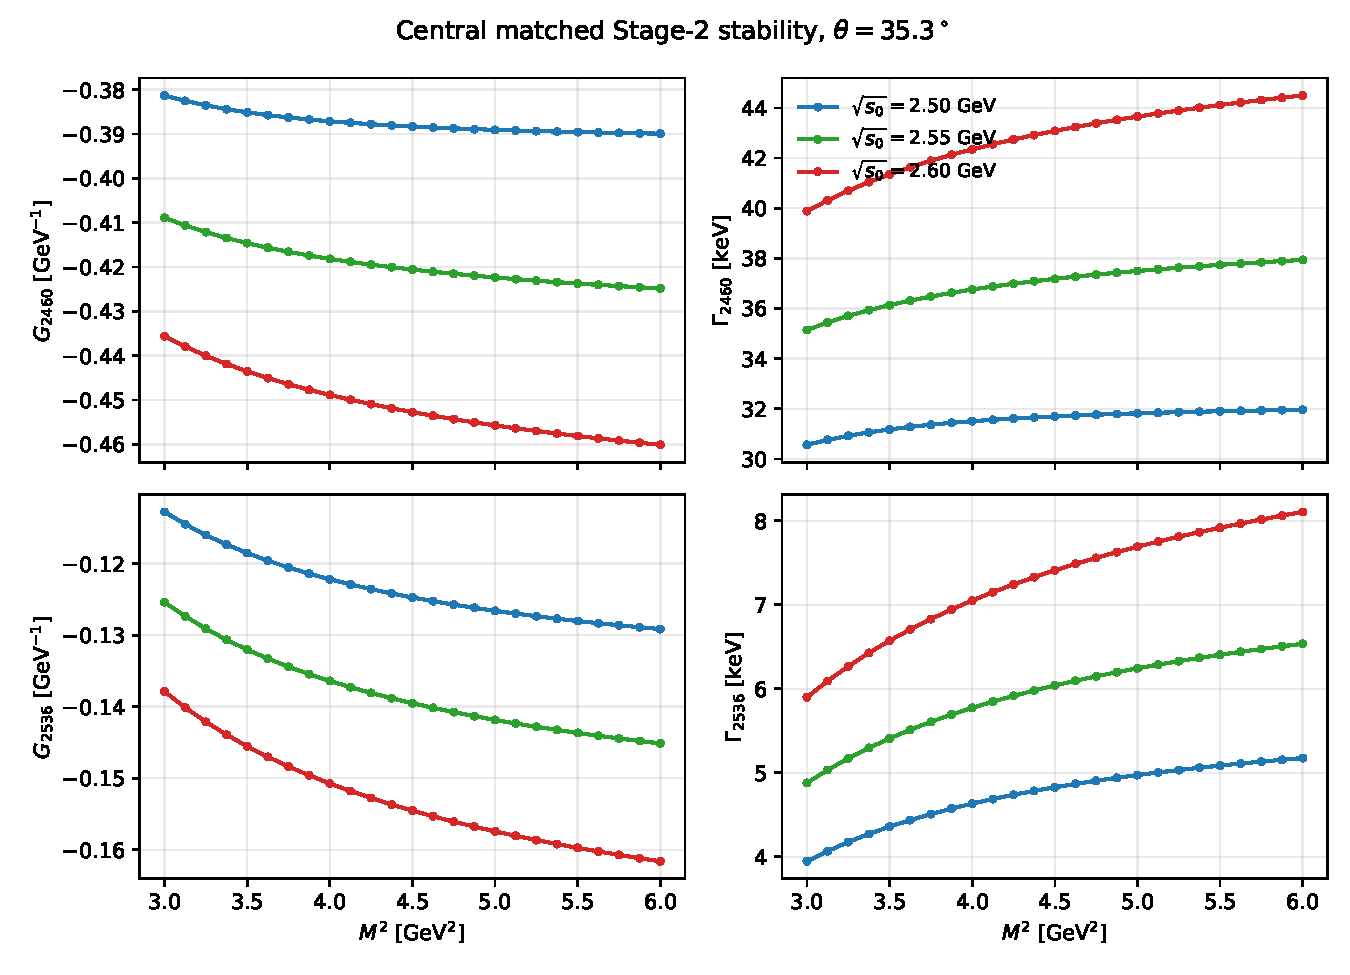
\includegraphics[width=0.95\textwidth]{../outputs/stage2_stability_central.pdf}
  \caption{Central matched Stage 2 stability for
  $\Dsone(2460)\to\Ds\gamma$ and $\Dsone(2536)\to\Ds\gamma$ at
  $\theta=35.3^\circ$.  The three curves correspond to
  $\sqrt{s_0}=2.50,2.55,2.60~\mathrm{GeV}$.}
  \label{fig:stage2-stability}
\end{figure}

Across the full displayed window the central ranges are
\begin{align}
  \Gamma[D_{s1}(2460)\to D_s\gamma]
  &=
  30.6\text{ to }44.5~\mathrm{keV},\\
  \Gamma[D_{s1}(2536)\to D_s\gamma]
  &=
  3.95\text{ to }8.10~\mathrm{keV}.
\end{align}
The corresponding amplitude spans are smaller:
\begin{align}
  G_{2460}
  &=
  -0.460\text{ to }-0.381~\mathrm{GeV}^{-1},\\
  G_{2536}
  &=
  -0.162\text{ to }-0.113~\mathrm{GeV}^{-1}.
\end{align}
This is the expected pattern: the widths amplify the residual sum-rule
variation because $\Gamma\propto G^2|\vec q|^3$.

\section{Publication Figures and Phenomenology}

The remaining publication-oriented figures are generated by
\begin{center}
  \texttt{scripts/publication\_plots.py}.
\end{center}
Figure~\ref{fig:threshold-dependence} shows the continuum-threshold
dependence at fixed representative values of $M^2$.  It complements
Fig.~\ref{fig:stage2-stability}: the curves are monotonic in $\sqrt{s_0}$, so
the continuum threshold should be quoted as an important systematic.

\begin{figure}[htbp]
  \centering
  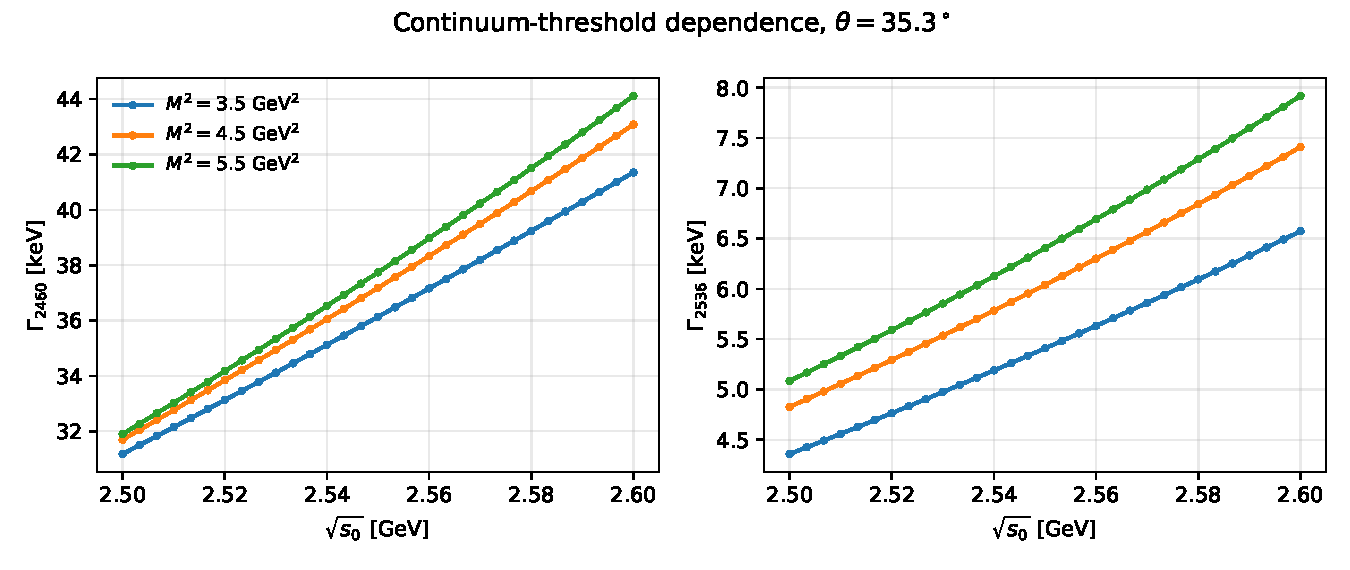
\includegraphics[width=0.95\textwidth]{../outputs/stage2_threshold_dependence.pdf}
  \caption{Continuum-threshold dependence of the matched Stage 2 widths for
  $\theta=35.3^\circ$ at three representative Borel points.}
  \label{fig:threshold-dependence}
\end{figure}

Figure~\ref{fig:mixing-dependence} shows the mixing-angle dependence.  The
$D_{s1}(2460)$ width remains at the tens-of-keV level over a broad range of
$\theta$, while the $D_{s1}(2536)$ width is strongly suppressed near the
large-angle region because its amplitude involves a cancellation between the
axial and tensor-current components.

\begin{figure}[htbp]
  \centering
  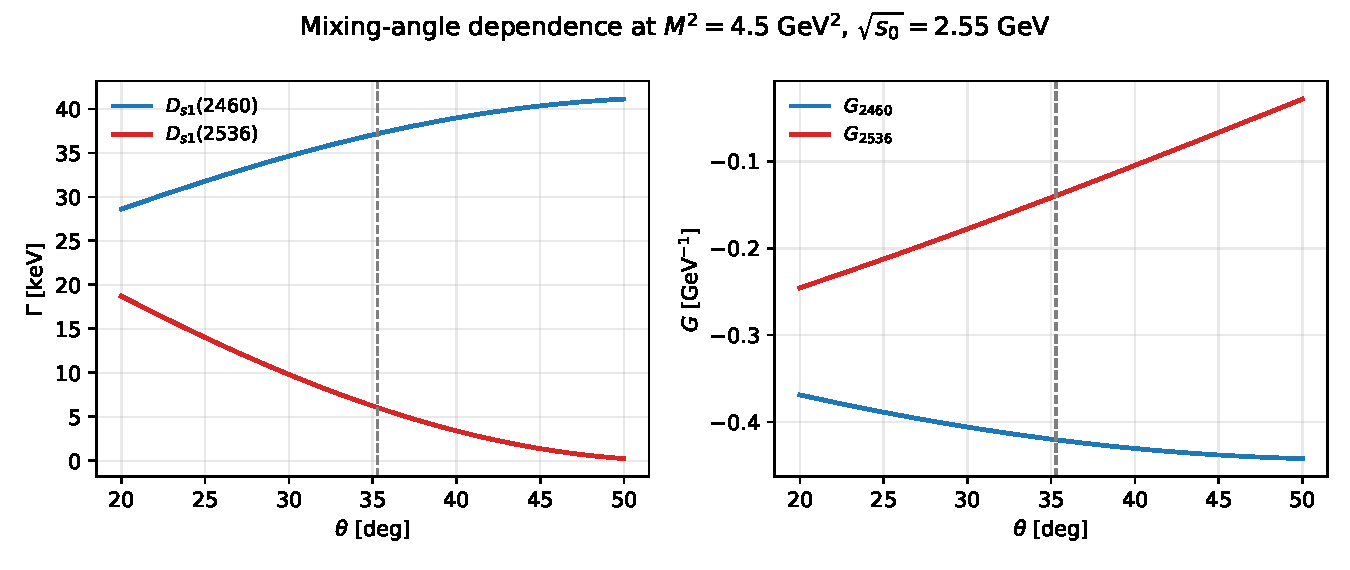
\includegraphics[width=0.95\textwidth]{../outputs/stage2_mixing_angle_dependence.pdf}
  \caption{Mixing-angle dependence at $M^2=4.5~\mathrm{GeV}^2$ and
  $\sqrt{s_0}=2.55~\mathrm{GeV}$.  The dashed line marks
  $\theta=35.3^\circ$.}
  \label{fig:mixing-dependence}
\end{figure}

The cancellation pattern is displayed more explicitly in
Fig.~\ref{fig:contribution-breakdown}.  At the central point
$M^2=4.5~\mathrm{GeV}^2$, $\sqrt{s_0}=2.55~\mathrm{GeV}$, the
$D_{s1}(2536)$ amplitude receives opposite-sign contributions from the axial
Stage 1 term and the hard tensor-current term.  The three-particle DA
corrections are numerically small in the final physical amplitudes, but they
are included in the quoted Stage 2 result.

\begin{figure}[htbp]
  \centering
  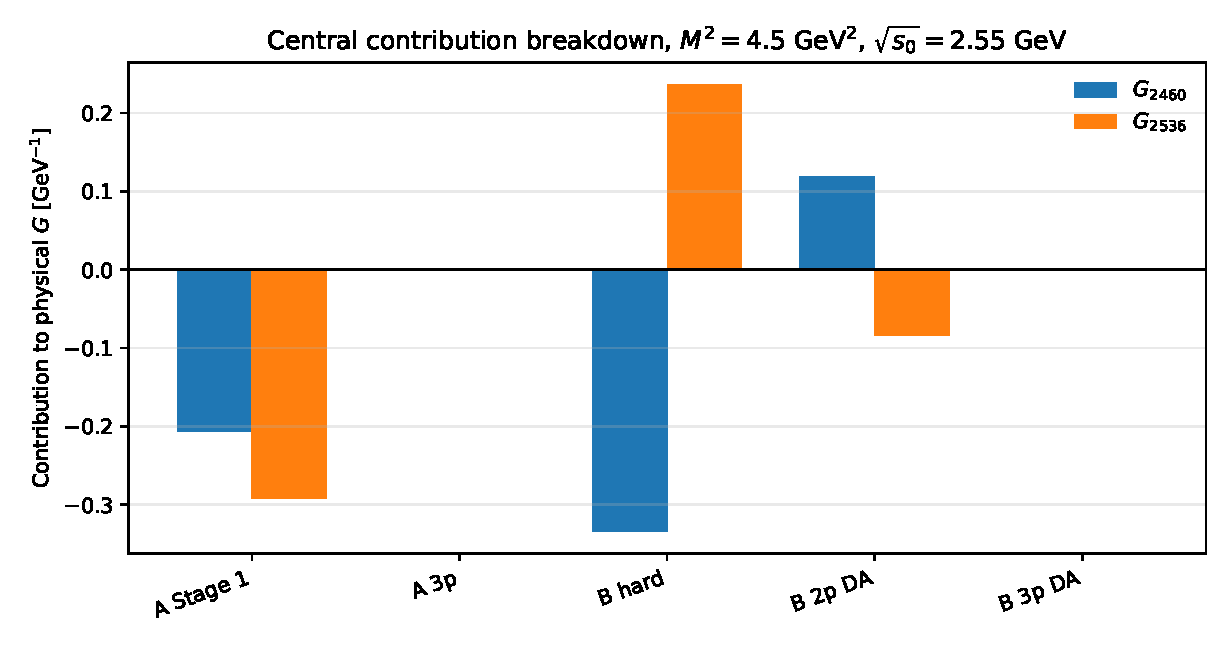
\includegraphics[width=0.95\textwidth]{../outputs/stage2_contribution_breakdown.pdf}
  \caption{Contribution breakdown for the physical couplings at the central
  Borel and threshold point.  The labels ``A'' and ``B'' refer to the
  axial-current and tensor-current components before physical mixing.}
  \label{fig:contribution-breakdown}
\end{figure}

Finally, Fig.~\ref{fig:literature-comparison} compares the present result for
$D_{s1}(2460)\to D_s\gamma$ with representative estimates collected by
Colangelo, De Fazio and Ozpineci.  The present result is higher than the
original axial-current LCSR interval, but it remains the same order of
magnitude.  It should not be advertised as explaining a non-observation by
making the $D_{s1}(2460)\to D_s\gamma$ width tiny.  Instead, the robust
phenomenological statement from this calculation is that the
$D_{s1}(2536)\to D_s\gamma$ channel is much more cancellation-sensitive and can
be substantially smaller.

\begin{figure}[htbp]
  \centering
  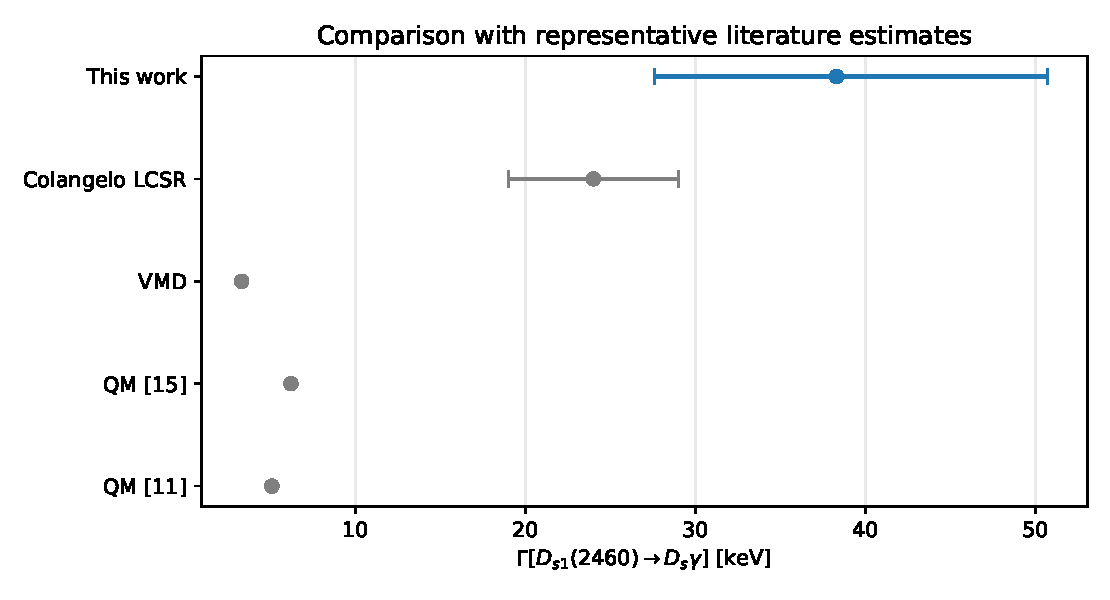
\includegraphics[width=0.82\textwidth]{../outputs/literature_comparison_2460.pdf}
  \caption{Comparison of the present $D_{s1}(2460)\to D_s\gamma$ width with
  representative literature estimates.  The Colangelo LCSR, VMD and quark-model
  values are from the comparison table in Colangelo, De Fazio and Ozpineci
  (hep-ph/0505195).}
  \label{fig:literature-comparison}
\end{figure}

\section{Validation Checks Before the \(B_{s1}\) Extension}

The script
\begin{center}
  \texttt{scripts/validation\_checks.py}
\end{center}
collects several checks that should be repeated whenever the numerical
implementation is modified.  The first check is an axial-current benchmark
against Colangelo, De Fazio and Ozpineci, using paper-like input choices and
the BBK value $\kappa=0.2$ for the relevant photon DA parameter.  Over
$3\leq M^2\leq 6~\GeV^2$ and
$2.50\leq \sqrt{s_0}\leq2.60~\GeV$, the present controlled benchmark gives
\begin{equation}
  g_1=-0.340\text{ to }-0.237~\GeV^{-1},\qquad
  \Gamma=11.8\text{ to }24.3~\mathrm{keV}.
\end{equation}
The published comparison band is
$g_1=-0.37\text{ to }-0.29~\GeV^{-1}$ and
$\Gamma=19\text{ to }29~\mathrm{keV}$.  This is close enough in sign and
scale to validate the implementation, but it also shows that an exact
literature reproduction requires matching every convention and input choice.
We should present this as a benchmark check, not as an independent final
phenomenological result.

The same validation script checks the photon DA normalization and the
three-particle integration closure:
\begin{align}
  \int_0^1 du\,\varphi_\gamma(u)&=1.0000000000,\\
  \max_u|\psi^a(u)-\psi^a(1-u)|&=4.44\times 10^{-15},\\
  \max_u|\psi^v(u)+\psi^v(1-u)|&=1.78\times 10^{-15},\\
  F_1-F_1^{(1)}-F_1^{(2)}&=0.
\end{align}
These are numerical quadrature checks of the DA implementation and the split
integration domains.

The independent FeynCalc script
\texttt{scripts/ward\_transversality\_check.wl} checks the selected E1 tensor
$S_{\mu\nu}=p_\nu q_\mu-(p\cdot q)g_{\mu\nu}$.  With
$q^2=0$, $\varepsilon\cdot q=0$, $P=p+q$, and $\eta\cdot P=0$, it gives
\begin{align}
  S_{\mu\nu}q^\nu &=0,\\
  \left[(\eta\cdot\varepsilon)(p\cdot q)
    -(\eta\cdot q)(p\cdot\varepsilon)\right]_{\varepsilon\to q}
  &=0,\\
  P^\mu S_{\mu\nu}\varepsilon^\nu&=0,\\
  \frac{S_{\mu\nu}S^{\mu\nu}}{2(p\cdot q)^2}&=1.
\end{align}
The first two equations are the photon Ward check, the third confirms
compatibility with the physical initial axial-meson polarization, and the last
line is the projector normalization.

At the central point $M^2=4.5~\GeV^2$ and
$\sqrt{s_0}=2.55~\GeV$, the hard tensor-current charge decomposition is
\begin{align}
  G_B^{\mathrm{hard}}&=-4.092\times10^{-1}~\GeV^{-1},\\
  G_B^{\mathrm{hard}}(e_c\text{ line})&=-2.499\times10^{-1}~\GeV^{-1},\\
  G_B^{\mathrm{hard}}(e_s\text{ line})&=-1.594\times10^{-1}~\GeV^{-1}.
\end{align}
This confirms that hard photon emission from both quark lines is numerically
important and must remain in the baseline.

\begin{table}[htbp]
  \centering
  \begin{tabular}{lrrrr}
    \toprule
    Diagnostic case & $G_A$ & $G_B$ & $\Gamma_{2460}$ & $\Gamma_{2536}$\\
    & \multicolumn{2}{c}{($\GeV^{-1}$)} & \multicolumn{2}{c}{(keV)}\\
    \midrule
    central & $-0.357$ & $-0.263$ & $37.18$ & $6.04$\\
    $m_s\to0$ numerical proxy & $-0.175$ & $-0.210$ & $15.59$ & $0.15$\\
    $m_s=m_c$ toy & $+0.535$ & $+0.273$ & $59.46$ & $24.22$\\
    $e_c=0$ toy & $+0.102$ & $-0.013$ & $0.50$ & $2.57$\\
    $e_s=0$ toy & $-0.459$ & $-0.250$ & $46.30$ & $16.48$\\
    light-$u$ OPE toy & $-1.040$ & $-0.438$ & $192.96$ & $110.02$\\
    light-$d$ OPE toy & $-0.109$ & $-0.176$ & $8.94$ & $0.05$\\
    \bottomrule
  \end{tabular}
  \caption{Limiting-case diagnostics from
  \texttt{outputs/validation\_limiting\_cases.csv}.  The $m_s\to0$ and
  light-quark rows use $m_q=10^{-4}~\GeV$ as a numerical regulator of the
  present hard-line spectral-density representation.  The light-$u$ and
  light-$d$ rows are OPE-level charge and condensate substitutions only, not
  physical nonstrange $D_1\to D\gamma$ predictions.}
  \label{tab:validation-limits}
\end{table}

\section{Missing Or Useful Paper Material}

Before moving from the $D_{s1}$ paper draft to the $B_{s1}$ extension, the
following items are useful to add or verify.

\begin{itemize}
  \item A compact input table in the paper text: masses, decay constants,
  condensates, $\chi$, DA parameters, Borel windows, and continuum thresholds.
  The final numerical scan already uses these values, but the paper needs a
  reader-facing table.
  \item A short paragraph on convention matching.  The sign of $\chi$, the
  Levi-Civita convention, and the tensor-current normalization
  $f_B=f_Tm_{D_{s1}}/(m_c+m_s)$ should be stated explicitly because they move
  signs and absolute normalizations.
  \item A clearer uncertainty budget.  The current global scan varies
  $M^2$, $s_0$, $\chi$, decay constants, quark masses, condensates, and the
  mixing angle in the broad scan.  A one-at-a-time error table would show that
  the large uncertainty is driven mainly by mixing-angle and threshold
  sensitivity, not by missing ordinary condensate terms in the propagator.
  \item A physical light-quark counterpart requires new hadronic input tables.
  The OPE-level light-$u$ and light-$d$ diagnostics above are useful algebra
  checks, but physical $D_1\to D\gamma$ or $B_1\to B\gamma$ predictions need
  the corresponding hadron masses, decay constants, thresholds, Borel windows,
  condensates, and mixing convention.
  \item For the $B_{s1}$ extension, the same code structure can be reused after
  replacing $m_c\to m_b$, $m_{D_s}\to m_{B_s}$,
  $m_{D_{s1}}\to m_{B_{s1}}$, and updating the tensor decay constant and
  threshold window.  The hard-photon terms should be recomputed rather than
  scaled by hand, because the charm and bottom propagator denominators weight
  the heavy-line emission differently.
\end{itemize}

\end{document}
